\documentclass[a0,portrait]{a0poster}

% --- Entrada / fontes ---
\usepackage[utf8]{inputenc}
\usepackage[T1]{fontenc}
\usepackage{lmodern}
\usepackage{xcolor}
\definecolor{myblue}{HTML}{2E326F}
\definecolor{myblue2}{HTML}{1F7A8C}
\definecolor{lightblue}{HTML}{EBF4F6} 
\definecolor{myred}{HTML}{840F1A}
\renewcommand{\familydefault}{\sfdefault}

% --- Básicos ---
\usepackage{graphicx}
% busca imagens na pasta imagens/
\graphicspath{{imagens/}}
\usepackage{amsmath,amssymb}
\usepackage{mathrsfs}
\usepackage{setspace}
\onehalfspacing
\usepackage[dvipsnames]{xcolor}
\usepackage{tikz}
\usepackage{eso-pic}
\usepackage{multicol}
\usepackage{float}
\usepackage{enumitem}
\newtheorem{teo}{Theorem}
\newtheorem{exe}{Example}
\newtheorem{lema}{Lemma}
\newcommand{\N}{{\rm {I\!N}}}
\newtheorem{defi}{Definition}
\setlength{\columnsep}{1.5cm}
\renewcommand{\normalsize}{\fontsize{35}{40}\selectfont} % 48pt fonte, 56pt espaçamento
\renewcommand{\Large}{\fontsize{45}{60}\selectfont\bfseries} % 60pt fonte para títulos menores
\renewcommand{\LARGE}{\fontsize{50}{70}\selectfont\bfseries} % 72pt fonte
\renewcommand{\large}{\fontsize{40}{50}\selectfont\bfseries}
\renewcommand{\huge}{\fontsize{70}{80}\selectfont\bfseries} % 84pt fonte
\renewcommand{\Huge}{\fontsize{80}{110}\selectfont\bfseries} % 96pt fonte

% --- Fundo: degradê vertical (azul escuro em cima -> azul claro em baixo) ---
\AddToShipoutPictureBG*{%
  \begin{tikzpicture}[remember picture,overlay]
    % Gradiente: branco forte no topo -> quase branco -> azul final
    \path[shade, shading=axis,
          top color=white,
          middle color=white,
          bottom color=lightblue]
      (current page.south west) rectangle (current page.north east);
  \end{tikzpicture}
}



% --- Estilo das seções (opcional) ---
\makeatletter
\renewcommand{\section}{\@startsection%
  {section}{1}{0mm}{-\baselineskip}{1mm}{\LARGE\color{myred}\bfseries}}
\renewcommand{\subsection}{\@startsection%
  {subsection}{2}{0mm}{-0.9\baselineskip}{1mm}{\Large\color{myred}\bfseries}}
\renewcommand{\subsubsection}{\@startsection%
  {subsubsection}{3}{0mm}{-0.7\baselineskip}{1mm}{\large\color{myred}\bfseries}}
\makeatother

\begin{document}

\begin{center}
\parbox{0.2\textwidth}{
\begin{center}
\hspace{10cm}
\includegraphics[scale=0.225]{brasao_UFSC.png}
\end{center}}
\parbox{0.40\textwidth}{
\begin{center}
\textrm{{\huge {\color{myblue} \textbf{
			Work Title}}}\\[1ex]
\bigskip
{\LARGE First Author Name $^1$ (University)}\\[1ex]
{\LARGE Co-author 1 Name (University)\\ 
	\vspace{0.2cm} Co-author 2  Name (University)}\\[1ex]
{\large First author e-mail$^1$}}\\[1ex]
\end{center}
}
\parbox{0.3\textwidth}{
\begin{center}
\includegraphics[scale=0.9]{ermac-logo-texto.pdf}
\end{center}}
\parbox{0.9\textwidth}{
\begin{center}
\large
 \textcolor{blue}{\section*{Abstract}}
 \end{center}
  \large
The general objective of this work was to perform a theoretical study about ...}
\end{center}
\vspace{2cm}
\begin{multicols}{2}
\section*{\textcolor{myblue}{Introduction}}
\textcolor{myblue}{
Briefly introduce the broad field of your research. E.g: Several fields of science make use of Optimization to aid in decision making. In particular, this is observed in ...
Cite like this~\cite{Reference4, Reference6}.
Example equation:
\begin{equation}\label{problema_geral}
\begin{array}{cl}
\displaystyle\min_{x}&f(x)\ \mbox{ with } x \in \mathbb{R}^n  \\
s.a & g(x)\leq 0,
\end{array}
\end{equation}
where the functions $f:\mathbb{R}^{n}\rightarrow\mathbb{R}$ and $g:\mathbb{R}^{n}\rightarrow\mathbb{R}$ are continuously differentiable.}
\section*{Methodology}
Figure Example:
\begin{center}
	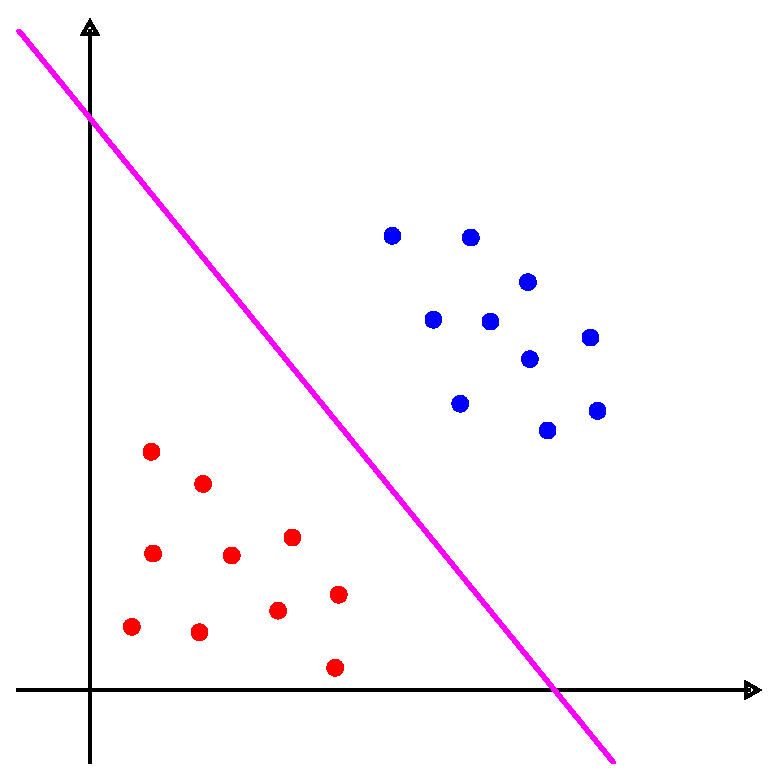
\includegraphics[scale=0.5]{svmfig2_margemrigida.eps}\hspace{1.5cm}
	\hspace{1.5cm}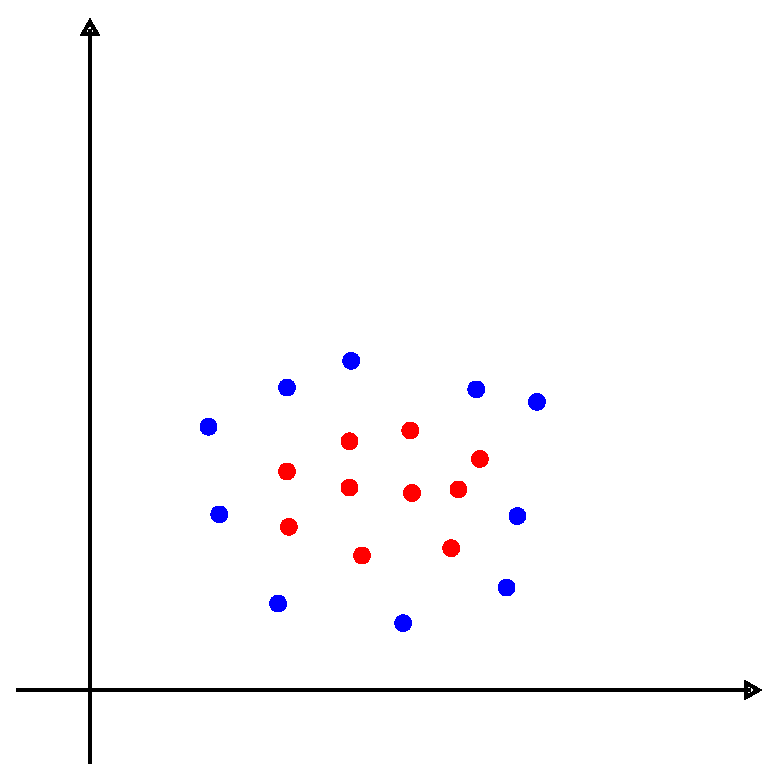
\includegraphics[scale=0.5]{svmfig2_naolinear.eps}
	\\
	\hspace{2cm}\textbf{Figure 1} \textcolor{myblue}{Linear.}\hspace{2cm}
	\hspace{1.5cm}\textbf{Figure 3}  \textcolor{myblue}{Non linear.}
\end{center}
\subsection*{Subsection 1}

\begin{teo}\label{teorema1}
	Consider the quadratic problem
	\begin{equation}
	\label{prob_quad}
	\begin{array}{cl}
	\displaystyle\min_x & f(x)=x^THx+c^Tx\\
	s.a & Ax+b\leq 0,
	\end{array}
	\end{equation}
	where $H\in\mathbb{R}^{n\times n}$ is symmetric, $c\in\mathbb{R}^n$, $A\in\mathbb{R}^{m\times n}$ 
	and $b\in\mathbb{R}^m$. Suppose that its feasible set
	is non-empty and that the objective function is bounded below in this set. So
	the problem has a global minimizer.
\end{teo}


\subsubsection*{Subsubsection (if necessary)}

For this problem, we can guarantee the existence of a solution for the specific case. We deal with obtaining .... because we can not guarantee ... has a unique solution and we show Example~\ref{analisevs} for which the dual has infinite solutions.
\begin{exe}
	\label{analisevs}
	Consider the following set, 
	... 
\end{exe}


In the light of this example, we present two definitions present in the literature ~\cite{Reference1, Reference2}.
\begin{defi}
	\label{def_vs1}
	Definition Example
\end{defi} 

\subsection*{Subsection 2}
\section*{Numerical Results}



\textcolor{myblue}{
\section*{\textcolor{myblue}{Conclusions}}
The main contributions of this work are:
\begin{itemize}
	\item Conclusion 1
	\item Conclusion 2.
	\item ....
	\item ....
	\item .....		
\end{itemize}
}	
\section*{Acknowledgements}
My teachers xxx and xxx. Supported by CAPES (Brazil).
\begin{thebibliography}{2}
	\bibitem{Reference1}C. M. Reference1, {\it Work Title}. Journal, Publisher, Volume, Number, Pages,  Year.
\bibitem{Reference2}N. Reference2 and J. Reference3,
\emph{Work Title}. Journal, Publisher, Volume, Number, Pages,  Year.
\bibitem{Reference4}V. N. Reference4 and I. M. Reference5, \textit{Work Title}. Journal, Publisher, Volume, Number, Pages,  Year.
\bibitem{Reference6}V. N. Reference6 and C. Reference7, \textit{Work Title}. SIAM Journal on Optimization, SIAM, v. 20, n. 3, pp. 273-297, 1995.

\end{thebibliography}
\end{multicols}
\end{document}